\chapter{Memory consolidation through combined burst-induced homeostatic reset and structural plasticity}
\begin{shaded}
BLA BLA

\end{shaded}

% -------------------------------
% -------------------------------
%
%        INTRODUCTION
%
% -------------------------------
% -------------------------------
\section{Introduction}
\textcolor{blue}{OCNS}\\
Neurons adapt their connections with each other through synaptic plasticity, driven by correlations in their spiking activity (Fig. 1A). Additionally, neuronal networks undergo global changes in rhythmic activity that correspond to different brain states, defined by switches in neuronal activity and orchestrated by neuromodulators. A well-known example is the transition from a state of learning during active waking to rest during quiet waking, which corresponds to a switch in neuronal activity from tonic firing to bursting (Fig. 1B). This raises the question of how switching from tonic firing to bursting affects the outcome of synaptic plasticity and whether it can support memory consolidation.
Recently, we have shown for a variety of synaptic plasticity models that bursting leads to a homeostatic reset, in which synaptic efficacy returns to a fixed baseline value irrespective of the starting point. This homeostatic reset causes the network to forget any learned information [1]. To address this issue, we propose an additional structural plasticity mechanism in which short-term changes in synaptic efficacy – evolving according to traditional plasticity rules – drive long-lasting morphological changes such as spine growth or insertion of new AMPA receptors. While synaptic efficacy undergoes homeostatic reset during bursting, information is consolidated through structural plasticity on a longer timescale.
We demonstrate the utility of this mechanism in a network of neurons using a conductance-based neuronal model that can switch from tonic firing to bursting along with a calcium-based synaptic rule to drive changes in synaptic efficacy. We investigate three regimes of switches in neuronal activity and plasticity mechanisms, denoted S1, S2, S3 (Fig. 1C). In S1, as a control condition, tonic firing is interleaved with periods of neuronal inactivity – mimicking bursting blockers – and a traditional plasticity rule, while in S2, tonic firing is separated by periods of bursting, leading to homeostatic reset in synaptic efficacy. Configuration S3 is identical as S2 but also includes our proposed burst-driven structural plasticity. 
In our first memory task (Fig. 1D), we show that the signal-to-noise (SNR) is improved over repeated switches only in S3. In a simple pattern recognition task (Fig. 1E), blocking bursting activity (S1) makes the network fragile to noise, and blocking structural plasticity during bursting leads to complete forgetting (S2), neither of which occurs in S3. Finally, in a MNIST recognition task (Fig. 1F), we confirm that memory consolidation occurs with S3 by showing a stronger receptive field that consolidates during switches from tonic to burst and is robust to noise. 
In this work, we shed light on the under-investigated role of switches in neuronal firing patterns for synaptic plasticity. Traditional plasticity rules result in a burst-induced homeostatic reset of synaptic efficacy, which is incompatible with memory consolidation. Our burst-driven structural plasticity proposes a solution to this problem, bridging the gap between switches in tonic firing to bursting, learning, and memory consolidation, and suggesting new ways to improve machine learning algorithms. 




% -------------------------------
% -------------------------------
%
%           METHODS
%
% -------------------------------
% -------------------------------

\section{Methods and Computational experiments}
\subsection{Conductance-based modeling}
\textcolor{blue}{same as reset}\\
\textcolor{orange}{est-ce que je le renote ici brèvement}

\subsection{Circuit architecture}
\textcolor{red}{parler du courant syn ou le mettre direct dans conductance-based modeling}
% -------------------------------
%     Traditional plasticity
% -------------------------------
\subsection{Synaptic plasticity}
\subsubsection{Definition of the synaptic strength}
The synaptic current between the excitatory presynaptic neuron and postsynaptic neuron is an AMPA current as $I_\mathrm{syn} = I_\mathrm{AMPA}$, defined by $I_\mathrm{AMPA} = wg s_\mathrm{AMPA}(V_\mathrm{m}-E_\mathrm{AMPA}$. The synapse is modeled by $wg$ called the effective synaptic weight where $w$ the  \textit{synaptic efficacy}, and $g$ is the \textit{synaptic conductance}. The variable $w$ is driven by traditional synaptic plasticity rules. We compared the pair-based rule \citep{abbott_synaptic_2000} or the calcium-based plasticity rule \citep{graupner_natural_2016} \textcolor{magenta}{check for triplet?}. The variable $g$ is governed by a structural plasticity rule developed in this project (explained in the following section).

\subsubsection{Calcium-based model}
\textcolor{blue}{la meme regle clacique que dans le reset}\\
\textcolor{orange}{est-ce que je le note}
\subsubsection{Pair-based model}
idem

% -------------------------------
%           Methods: structural plasticity
% -------------------------------

\subsubsection{Structural plasticity: plasticity on the synaptic conductance $g$}

The Late phase of Long-term plasticity relie on the generation of de novo proteins and morphological changes. These changes are encapsulated in a variable $g$, for simplicity called the synaptic conductance. The rule governing the change in this variable refers to structural plasticity. We developed a simple equation driven by the \textit{ homeostatic reset}, which is the result of the soft-bound traditional plasticity rule acting on $w$ during burst \citep{jacquerie_switches_2022}.  
This simple equation is written as
$$ \tau_g \dot{g} = \Delta g $$
where $\Delta g$ is comprised between -1 and 1 and decides if the conductance increases (positive value of $\Delta g$) or decreases (negative value of $\Delta g$). The term $\tau_g$ scales the speed of change is in order of magnitude of 1 to 10 seconds (\textcolor{blue}{add the exact value for each experiment in \textit{SI Appendix})}.


\textit{During bursting activity only}, the variable $\Delta g$ has the following dynamics: 
$$ \tau_\Delta \dot{\Delta g} = f(w) - \Delta g$$
where $\tau_\Delta$ is the time constant associated to the change in $\Delta g$ and $f(w)$ is a sigmoidal function between -1 and 1 written as:
$$ f(w) = -1+2\left( \frac{e^{\mathrm{slope} (w-w_\mathrm{HR})}}{1+e^{\mathrm{slope} (w-w_\mathrm{HR})}} \right) $$
where slope defines the steepness of the sigmoid (the largest the value, the steepest the transition from -1 to 1). The term $w_\mathrm{HR}$ is the homeostatic reset estimated each second during the bursting activity. 

For the calcium-based rule, the estimated reset value is computed by 
\begin{align}  w_\mathrm{HR} 
    & = \frac{ \Omega^\mathrm{d}\alpha^\mathrm{d} +\Omega^\mathrm{p}\alpha^\mathrm{p} }{\alpha^\mathrm{d} + \alpha^\mathrm{p}}.
\end{align}
where $\Omega^\mathrm{d}$ and $ \Omega^\mathrm{p}$ are respectively the depression and potentiation levels and the effective time spent in each region $\alpha^\mathrm{d}$ and $\alpha^\mathrm{p}$ are defined as the time spent balanced by the time-constant of potentiation/depression in the corresponding region (as demonstrated in \citep{jacquerie_switches_2022}).
~\\
~\\
\textcolor{magenta}{decide if we repeat the experiment for the phenomenological rule}\\
\color{gray}
For the pair-based rule, the estimated reset value is given by 
\[ w_\mathrm{HR} = \frac{\frac{A^+C^+}{A^-C^-}}{1+\frac{A^+C^+}{A^-C^-}}.\]
with $A^+$ and $A^-$ are the potentiation and depression parameters of the pair-based rule. $C^+$ is the average correlation value between pre- and post- spiking time trains and $C^-$ is the average value between the post- and pre- spiking time trains (as demonstrated in \citep{jacquerie_switches_2022}). 
\color{black}


The bursting rhythm dictates the value of the homeostatic reset. Since it can be influenced during the state for example by neuromodulators or connectivity increase, the estimated value of the reset is computed each second which is realistic as the interburst frequency is around \textcolor{magenta}{add the value}.

If the neuron is not bursting, $\tau_\Delta \dot{\Delta g} = -\Delta g$. This value is converging towards 0. It guarantees the conductance to remain unchanged during the other states - an assumption made in this project. 

\subsubsection{Regimes}
Table \ref{tab:SP_overview} summarizes the different combinations between the switches between the different firing patterns (tonic firing, inactive, burst) and the different synaptic plasticity rules. 

\begin{table}[h]
    \centering
    \begin{tabular}{l|l|l|l|l}
        Model     & bounds & $\dot{w}$  & $\dot{g}$ & switch\\
        \hline
         $\#$1   & soft &  $\tau_w \dot{w} = \Omega([\mathrm{Ca}]) -w$ & fixed value   & tonic-inactive\\
         $\#$2   & soft &  $\tau_w \dot{w} = \Omega([\mathrm{Ca}]) -w$ & fixed value   & tonic-burst\\
         $\#$3  & soft &  $\tau_w \dot{w} = \Omega([\mathrm{Ca}]) -w$ & $\tau_g \dot{g} = \Delta g$ & tonic-burst   \\
         $\#$4  & hard &  $\tau_w \dot{w} = \Omega([\mathrm{Ca}])$ & fixed value  & tonic-inactive  \\
         $\#$5 &hard &  $\tau_w \dot{w} = \Omega([\mathrm{Ca}])$ & fixed value  & tonic-burst  \\
    \end{tabular}
    \caption{Overview of the synaptic plasticity models}
    \label{tab:SP_overview}
\end{table}




% -------------------------------
%           Methods: computational expm
% -------------------------------
\subsection*{Computational experiments}
\label{sec:computaional_expm}


% - - - - - - - - - - - - - - - - - 
%           comp expm: Gonz
% - - - - - - - - - - - - - - - - - 
\subsubsection{Pairing neurons}
\textit{Network}\\
We reproduce a similar computational experiment as in \citep{gonzalez-rueda_activity-dependent_2018}. We build a 2-layer network with 100 input neurons connected to one output neuron. An inhibtory neuron is connected via GABA\textsubscript{A} and GABA\textsubscript{B} currents to all the excitatory neurons with a fixed connectivity.\\
~\\
\textit{Simulations of the different states}\\
The network has three possible states: tonic firing, bursting, inactive.
\begin{itemize}
\item[-] During the tonic-firing learning state, we pair 5 of the 100 presynaptic neurons with the postsynaptic neuron by driving them with correlated inputs. The active input neuron receives a depolarizing current of 50 nA/cm$^2$ during 3ms at a frequency of $f_0 = 60$ Hz. The output neuron receives a similar input at $f_0 =40 $ Hz \citep{gurunathan_spurious_2020}. This input is sufficient to generate an action potential in the conductance-based model. To build a more realistic simulation, the spike timings are generated with interspike intervals following independent Normal distributions $\mathcal{N}(\frac{1}{f_0}, (\frac{\num{0.1}}{f_0})^{2})$. The 95 non correlated input neurons are stimulated in the similar manner except that the frequency $f_0$ is chosen between the following values (0.1, 0.25, 0.5, 0.75, 1, 1.25, 1.5, 2) Hz  from a uniform distribution. The output neuron is stimulated with a pulse train at 40Hz whose interspike intervals follow independent Normal distribution $\mathcal{N}(\frac{1}{f_0}, (\frac{\num{0.1}}{f_0})^{2})$.
\item[-] During bursting, the inhibitory cell is hyperpolarized with an external applied current equal to -1.2 nA/cm$^2$. 
\item[-] During inactive state, the neurons are driven with an applied current generating pulse at a frequency $f_0$ chosen in the range (0.1, 0.5, 1) Hz.   The spike timings are generated in the same manner following independent Normal distributions  $\mathcal{N}(\frac{1}{f_0}, (\frac{\num{0.1}}{f_0})^{2})$. 
\end{itemize}
\textcolor{red}{in Appendix SI -- } provide a table with the different value of the parameter used for the synaptic plasticity rules. \\
~\\
\textit{Protocols}\\
We record the evolution of the efficacy and the conductance during five cycles that is alternating between a tonic-firing learning state with either an intermittent bursting state or an inactive state without bursting. Each state lasts 15 seconds.

~\\
\textit{Analysis}\\
To analyse the evolution of the effective synaptic throughout the simulation, we compute the Signal-to-Noise Ratio (SNR) at the end of each state. The SNR is computed according to \citep{gonzalez-rueda_activity-dependent_2018}; $\mathrm{SNR} = \mathrm{max}(w)/\mathrm{mean}(w)$. \textcolor{red}{ce n'est pas wg ? }



% - - - - - - - - - - - - - - - - - 
%           comp expm: Gonz
% - - - - - - - - - - - - - - - - - 
\subsubsection{Pattern recognition}
\textcolor{red}{ref} \citep{fauth_self-organized_2019}, ...\\
In the pattern recognition task, we build a network of 9 presynaptic neurons connected to two postsynaptic neurons. The network learns to identify two patterns created in 3x3 pixel grid. Each pixel is associated to its own input neuron. An inhibtory neuron is connected via GABA\textsubscript{A} and GABA\textsubscript{B} currents to all the excitatory neurons with a fixed connectivity.\\
~\\
\textit{States}\\
The network can be in four different states: 
\begin{itemize}
    \item[-] learning state: inputs neurons are driven with an external current according to the pattern. If the pixel is active, the associated input neuron receives a applied current as a pulse at a frequency $f_0$ chosen in a normal distribution $\mathcal{N}(55$Hz$, 10)$. The amplitude of the pulse is equal to 50nA/cm$^2$ and the duration is equal to 3ms. To mimic a less regular spiking trains, the interspike interval is obtained in $\mathcal{N}(\frac{1}{f_0}, (\frac{\num{0.1}}{f_0})^{2})$. If the pixel is inactive, a similar stimulation is applied for a frequency $f_0$ chosen in a normal distribution $\mathcal{N}(1$Hz$, 0.01)$. The output neuron associated to the presented pattern is stimulated with a pulse train at $f_0$ = 40Hz whose interspike intervals follow independent Normal distribution $\mathcal{N}(\frac{1}{f_0}, (\frac{\num{0.1}}{f_0})^{2})$. The other neuron has a similar pulse train except that $f_0 = 0.01$Hz.  
    \item[-] bursting state: the inhibitory neuron is hyperpolarized by a current of -1.2nA/cm$^2$.
    \item[-] inactive state: all excitatory neurons are inactive and receive a pulse train at a frequency $f_0$ chosen in a normal distribution $\mathcal{N}(1$Hz$, 0.1)$.
    \item[-] noisy state: to mimic a noisy state, all neurons receive a pulse train at a frequency $f_0$ chosen in a normal distribution $\mathcal{N}(15$Hz$, 10)$. 
\end{itemize}
~\\
\textit{Protocols}\\
We build the following protocol in order to compare the different models with and without the structural plasticity rule and the effect of bursting state. The network sees 20 consecutive states. 
During the 12 first ones, learning state is interleaved by bursting state (for Models $\#$2, 3 and 5). The thirteenth state is the noisy state followed by a bursting state (for Models $\#$2, 3 and 5). The last part of the simulation is composed of succession between inactive states and bursting state (for Models $\#$2, 3 and 5). To study the impact of burst in the simulation, we reproduce the same protocol by replacing all the bursting states by resting states  (for Models $\#$ 1 and 4). 
During learning, we decide to either show one sample of the first pattern half of the state followed by one sample of the second pattern or we show two samples of the same pattern. Each state lasts 15s. \textcolor{red}{VERIFIER SI C'EST BIEN CA QUE JE FAIS ou plutot 1-3-4-7-9-10 pour pattern 1}. 
~\\
\textit{Testing}\\
The network has been simulated with the same protocol and the same samples for each synaptic plasticity models. To test their ability to recognize the two patterns, we create 50 samples of the first pattern and 50 samples of the second pattern. To build this sample, each active pixel (associated to the pattern) is firing according to a pulse train at a frequency $f_0$ chosen in a normal distribution $\mathcal{N}(65Hz,10)$. Each inactive pixel is stimulated in a similar manner at a frequency $f_0$ of $\mathcal{N}(2Hz,1.5)$.

Each pattern is shown 1s and we count the number of spikes of the two output neurons. We reproduce this process in the network with a fixed connectivity whose the value of $w$ and $g$ are retrieved from the simulation after each state. 

During testing, the output neurons are not stimulated. 

\textcolor{red}{ajouter la partie ou on ne teste que trois pixels sur 4}\\


\textcolor{magenta}{ajouter la partie ou on fait de l'overlap? }



~\\
\textit{Analysis}\\
description of prediction and certainty\\
\textcolor{red}{wait for the discussion with Dan - GD}\\
~\\
More details on all computational experiments can be found on \textit{SI Appendix}.


% - - - - - - - - - - - - - - - - - 
%           comp expm: MNIST
% - - - - - - - - - - - - - - - - - 
\subsubsection{MNIST}
\textit{Dataset/network}\\
~\\
\textit{States}\\
~\\
\textit{Protocols}\\
~\\
\textit{States}\\
~\\




% -------------------------------
% -------------------------------
%
%           RESULTS
%
% -------------------------------
% -------------------------------

\section{Results}
% -------------------------------
%           RESULT 1
% -------------------------------
\subsection{Structural plasticity prevents forgetting due to burst-induced homeostatic reset}

\textcolor{red}{ajouter la description pour les hard bounds}\\
As a simple testbed, we consider a circuit consisting of three biophysical conductance-based model neurons: an excitatory AMPA neuron (pre) synapsing onto another excitatory neuron (post), and an inhibitory GABA neuron synapsing onto both. Applying a hyperpolarizing current to the inhibitory cell models the effect of neuromodulators and switches the network state from tonic firing to bursting. The “post” neuron receives current from the “pre” neuron in proportion to the synaptic \textcolor{cyan}{conductance} $g$ (e.g. the number of AMPA receptors or the size of the dendritic spine) and synaptic \textit{efficacy} $w$ (e.g. the efficacy of AMPA receptors), such that the effective $synaptic weight$ is their product $wg$ (Fig. 1A). Traditional plasticity rules \citep{song_competitive_2000, graupner_natural_2016, pfister_triplets_2006} propose plasticity dynamics $\dot{w}$ to update the synaptic efficacy w and have been previously validated in this model on experimental data \citep{sjostrom_rate_2001, bi_synaptic_1998}. These traditional rules accurately explain change in synaptic efficacy $w$ that are independent on de novo protein synthesis, often referred as \textit{early phase Long Term Potentiation }(E-LTP) \citep{lamprecht_structural_2004}. 

To explore the interaction between synaptic plasticity and global brain states, we define three neuronal firing patterns; inactive , tonic firing (correlated or uncorrelated between pre and postsynaptic neurons for mimicking learning or not) or bursting (Fig. 1B). We simulate the network in a tonic state with a calcium-based plasticity driving change in synaptic efficacy \citep{graupner_natural_2016}. This state mimics a learning state by driving the excitatory neurons with either correlated or uncorrelated inputs (Fig. 1C, blue panels). As expected, strongly correlated neurons increase their efficacy (black curve), while weakly correlated ones have unchanged or decreased efficacy (Fig. 1C, gray curves). We then explore how learning is affected when tonic firing is followed by another firing pattern. In S1, when neurons switch from tonic firing to an inactive state, the weights remain unchanged. This illustrates a situation where bursting is blocked, for example in absence of external stimulus or in the presence of neuromodulator blockers (Fig. 1C, left). However, when switching from tonic firing to bursting (S2), homeostatic reset occurs, and the synaptic efficacy returns to its baseline, regardless of its learned value (Fig. 1C, center). This means that switching into a brain state driven by low-frequency oscillation, characterized by bursting activity at the neuronal level, erases all information previously stored in the synaptic efficacy value. This phenomenon was shown to be robust to intrinsic neuron variabilities, network heterogeneity and neuromodulation \citep{jacquerie_switches_2022}.


To address this issue with traditional plasticity rules on $\dot{w}$ and their limited ability to consolidate memory, we propose a mechanism of structural plasticity through dynamics in the synaptic conductance, $\dot{g}$, referred to \textit{late phase Long Term Potentiation} (L-LTP). This type of plasticity, which is protein-synthesis dependent, is associated with long term changes \citep{lamprecht_structural_2004, abraham_is_2019}. Although $w$ undergoes homeostatic reset as before, $g$ consolidates learned information. If the synaptic efficacy $w$ is higher than its reset value, the conductance $g$ increases through spine growth or insertion of new synthesized receptors (S3). Conversely, if $w$ is lower than its reset value, $g$ decreases through down-selection (Fig. 1C, right). Our work offers insights into the potential of incorporating structural plasticity during burst for improved memory consolidation, while the rest of the network weights return to baseline and are available for future learning. 


\begin{figure}
    \centering
    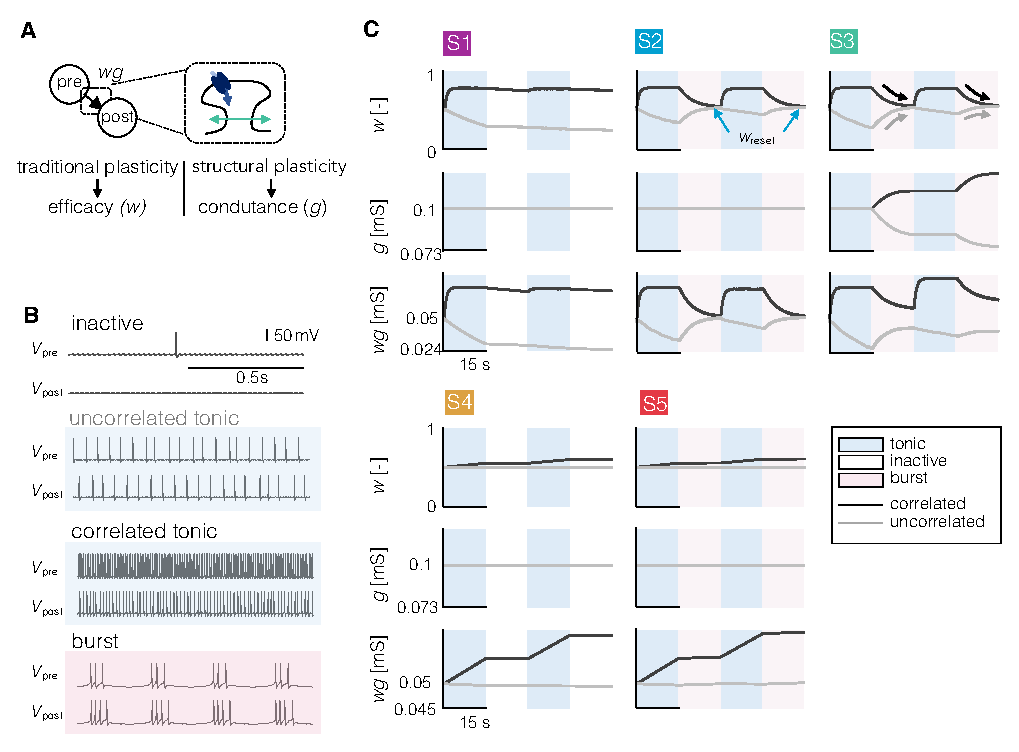
\includegraphics{fig/Task/Fig1.eps}
    \caption{Caption}
    \label{fig:Task_1}
\end{figure}


% -------------------------------
%           RESULT 2
% -------------------------------
%\subsection{Learning consolidates during burst through structural plasticity}
\subsection{Homeostatic reset and structural plasticity work together for memory consolidation}
We consider three memory tasks and compare the effect of different configurations of switches with their associated plasticity mechanisms. 

In the first memory task (Fig. 1D), as in \citep{gonzalez-rueda_activity-dependent_2018}, we pair five of 100 presynaptic neurons with a single postsynaptic neuron by driving them with correlated inputs in a tonic firing learning state. The remaining presynaptic neurons are uncorrelated. We repeated this procedure five times with either intermittent inactive states (S1) or bursting states (S2-S3). We find that only burst-driven structural plasticity paired with the homeostatic reset (S3) shows an increasing signal-to-noise (SNR) in the synaptic weights, over the course of multiple states. Suppressing bursting (S1) prevents the homeostatic reset but saturates the SNR at its steady-state value, while the calcium-based rule alone leads to forgetting through burst-induced homeostatic reset (S2). 



\begin{figure}
    \centering
    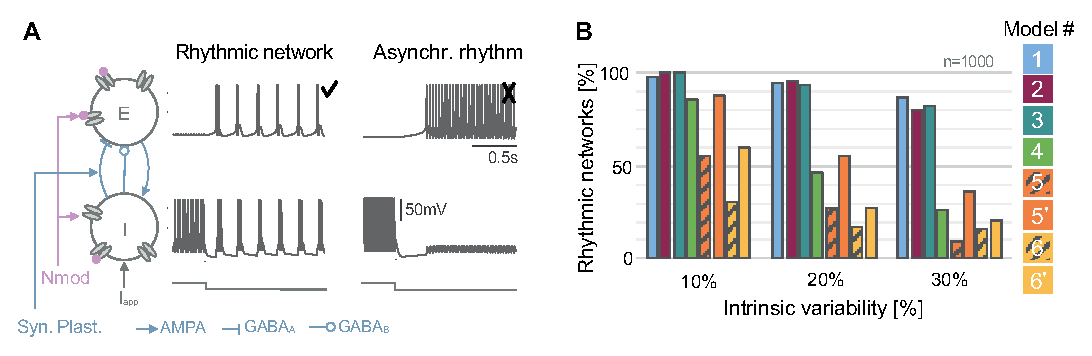
\includegraphics{fig/Task/Fig2.eps}
    \caption{Caption}
    \label{fig:Task_2}
\end{figure}


\begin{figure}
    \centering
    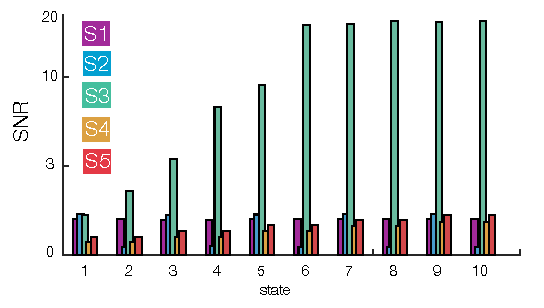
\includegraphics{fig/Task/Fig2_bar}
    \caption{Caption}
    \label{fig:Task_2_bar}
\end{figure}


% ---------------------------------------
%       RESULT 3: Pattern 
% ---------------------------------------
In the second memory task, we design a pattern recognition task (Fig. 1E), in which the network learns to identify two patterns, A and B. Each pixel of the grid is associated to one input neuron \citep{gurunathan_spurious_2020}. To emulate a variety of patterns, an input neuron which is associated to a pixel belonging to the pattern is tonically firing around 55Hz, while the other pixels are firing around 1Hz. During the tonic firing learning state, each pattern is paired with a corresponding output neuron. Learning states are interleaved with either inactive (S1) or bursting states (S2-S3) as in the first task. To test the robustness of the network to interference, we also add a noisy state in which neurons are tonically firing around 15Hz. During testing, we present either pattern A or B, which should cause only the corresponding output neuron to fire. The performance is computed after each state switch, and corresponds to the percentage of recognized patterns. We see that the burst-driven structural plasticity rule paired with the homeostatic reset (S3) allows memory consolidation and shows improved robustness to noise compared to the two other cases (S1-S2). In S1, the network, which illustrates the interaction between switches in tonic firing and a traditional synaptic plasticity rule alone, entirely forgets any learning as soon as noisy patterns are shown. In S2, once again we observe that each bursting state resets any learning. 

\textcolor{red}{ajouter la partie overlap ? et reconnaissance 3 digits? }


\begin{figure}
    \centering
    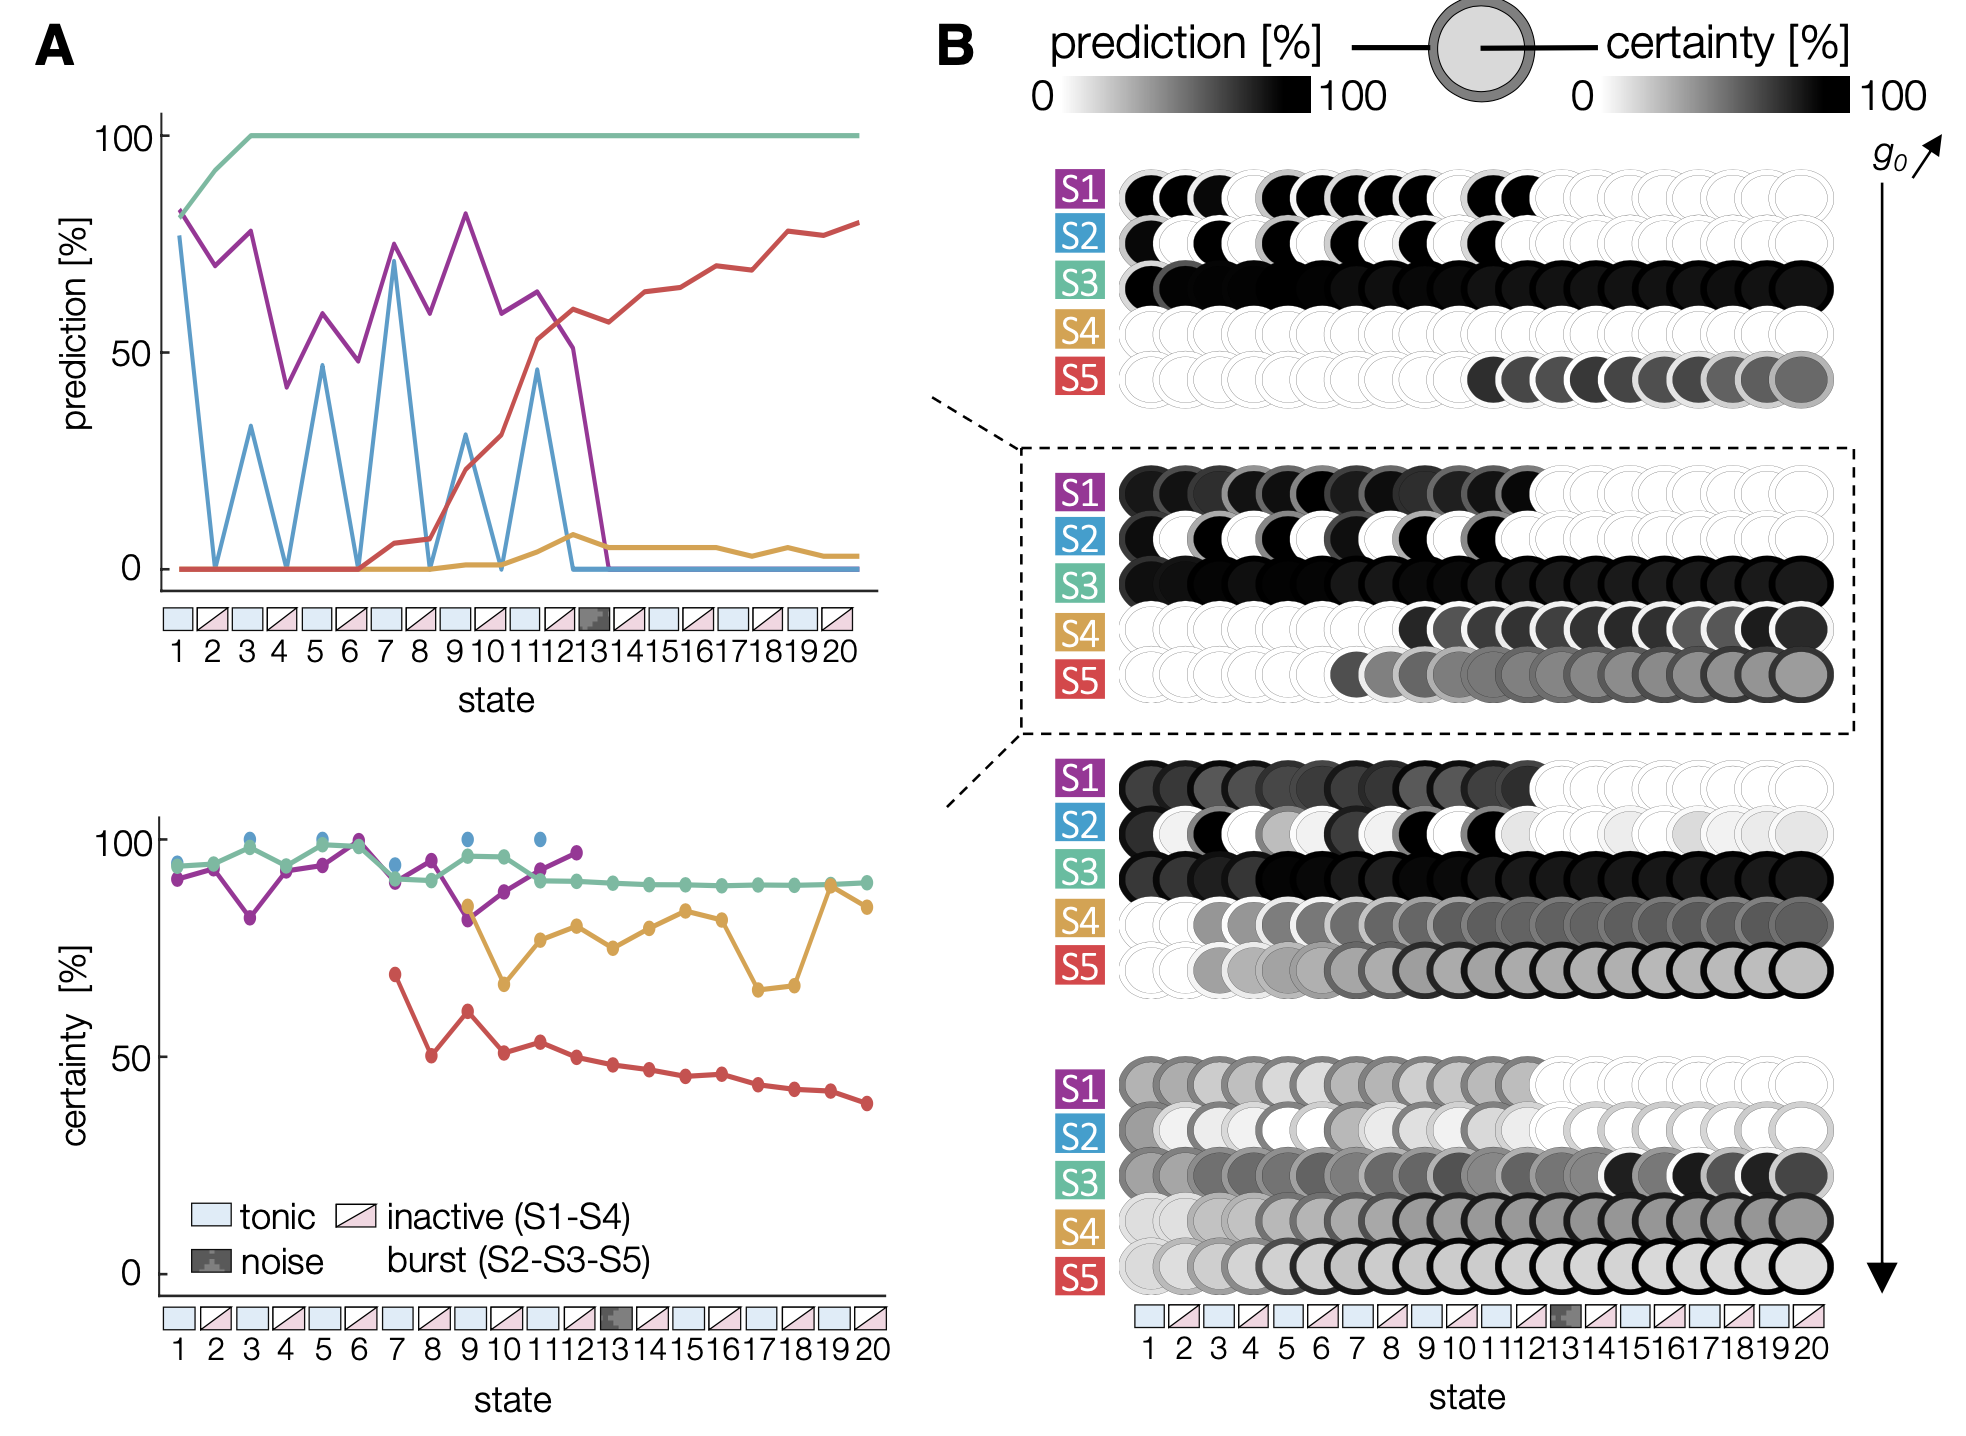
\includegraphics[scale=0.4]{fig/Task/Fig3_flake.png}
    \caption{Caption}
    \label{fig:Task_3_flake}
\end{figure}



% ---------------------------------------
%       RESULT 4: MNIST 
% ---------------------------------------
In the third memory task, we implement a more complex pattern recognition task using a reduced MNIST dataset \citep{garg_voltage-dependent_2022}. Again, we use tonic learning states interleaved with either inactive (S1) or bursting states (S2-S3). The \textit{receptive field} is defined as a weight matrix associated with each output neuron, which indicates the relative weights assigned to the input neurons contributing to that neuron's activation. We show the evolution of the receptive field of the output neuron associated to the digit 0 \textcolor{red}{modifier pour montrer tous les receptive fields}. We find that in S1, the receptive field is affected by each tonic firing learning state and entirely destroyed when a noisy image is presented. In S2, the receptive field resets at each bursting state as before. However, in S3, where learning is transferred from the synaptic efficacy to synaptic conductance, the receptive field is consolidated at each state and is robust to noise. 


% ---------------------------------------
%       RESULT 5: CONNECTIVITY 
% ---------------------------------------
\textcolor{red}{est-ce qu'on parle de ca ? }

% -------------------------------
% -------------------------------
%
%           DISCUSSION
%
% -------------------------------
% -------------------------------

\section{Discussion}
\subsection{Discussion 1}
\textcolor{blue}{COSYNE}\\
In summary, we show that traditional plasticity rules suffer from forgetting through burst-dependent reset but structural plasticity rescues memory and, combined with burst-induced reset, provides a robust mechanism for consolidation. Importantly, the results from our simple memory tasks make quantitative experimental predictions for the role of bursting states during learning. Finally, our work suggests incorporating structural plasticity and distinct tonic/bursting states for more reliable learning performance in artificial neural networks for machine learning applications. 



\textcolor{blue}{OCNS}\\
Overall, we demonstrate that while traditional plasticity rules enable learning during tonic states, they also result to forgetting due to homeostatic reset during bursting states. On the other hand, burst-driven structural plasticity salvages memory and, in combination with the homeostatic reset, provides a robust mechanism for consolidation. Moreover, when bursting states are replaced by inactive states, learning can be maintained but the SNR becomes saturated, memory consolidation is not achieved, and the network becomes vulnerable to noise (S1). Importantly, our results, which are based on simple memory tasks, generate quantitative experimental predictions for the role of bursting in learning. This confirms that synaptic plasticity is a complex process that operates on different timescales to facilitate memory formation and consolidation during switches in neuronal activity. Ultimately, our study suggests incorporating structural plasticity and distinct tonic/bursting states for more reliable learning performance in artificial neural networks, particularly in machine learning applications. 


\subsection{Limitations of the burst-dependent structural plasticity}
\textcolor{blue}{new}\\
Discuss the assumption made that $g$ is modified only during bursting rhythm and not in the other states. (i) justify with neuromodulator states, (ii) say that it is an assumption and to improve the structural plasticity, the synaptic conductance must change depending on internal state variable such as calcium for example. (iii) use a structural plasticity that is governed by $\dot{w}$ to avoid predicting the value of the reset. 


\section{Papers intéressants pour l'article}
- \citep{brokaw_resting_2016} "These observations suggest that a short period of quiet rest can facilitate memory consolidation processes."
- \textcolor{red}{retrouver l'article de Alessio qui montre que sans burst on n'a pas d'apprentissage}

